\documentclass{./springer/svjour3}
\usepackage{graphicx} % This lets you include figures
\graphicspath{ {./figures/} }
\usepackage[rightcaption]{sidecap}
% \usepackage{subcaption}
\usepackage{wrapfig}
\usepackage{float}
\usepackage{imakeidx}
\usepackage{comment}
\usepackage{commath}
\usepackage[titletoc]{appendix}
\usepackage{graphicx}
\usepackage{resizegather}
\usepackage[english]{babel}
% \usepackage{subcaption}
\usepackage{tabu}
\usepackage{booktabs}
\usepackage{xfrac}
\usepackage{tabularx}
% \usepackage{amssymb}
\usepackage{amsmath}
% \usepackage{amsthm}
\usepackage{commath}
\usepackage{graphicx,bm}
\usepackage{verbatim}
% \usepackage{caption}
\usepackage{lscape}
\usepackage{relsize}
\usepackage{enumitem}
\usepackage{textcomp}
\usepackage{breqn}
\usepackage{makecell}
\usepackage{longtable,tabularx}
\usepackage{multirow}
\usepackage{doi}
\usepackage{fancyhdr}
\usepackage{algorithm}
\usepackage{algpseudocode}
\usepackage{setspace}
\usepackage{footnote}
\PassOptionsToPackage{hyphens}{url}
\usepackage{hyperref}
\hypersetup{colorlinks,linkcolor={blue},citecolor={blue},urlcolor={blue}}
\usepackage[numbers]{natbib}
\usepackage{mathtools}
%\usepackage[disable]{todonotes}
\usepackage[framemethod=tikz]{mdframed}
\usepackage{booktabs,xcolor,siunitx}
\usepackage{soul}
% \usepackage{cleveref}
\usepackage[small, compact]{titlesec}
\usepackage{xcolor}
\usepackage{appendix}
% \usepackage{geometry}
% \geometry{
% a4paper,
% total={170mm,257mm},
% left=20mm,
% top=20mm,
% }

% \newtheorem{theorem}{Theorem}[section]
% \newtheorem{lemma}[theorem]{Lemma}
\newcommand{\ra}[1]{\renewcommand{\arraystretch}{#1}}
\newcommand{\degree}{\ensuremath{^\circ\,}}
\newcommand{\overbar}[1]{\mkern 1.5mu\overline{\mkern-1.5mu#1\mkern-1.5mu}\mkern 1.5mu}
\newcommand{\f}[2]{\frac{#1}{#2}}
\newcommand{\mb}[1]{\mathbf{#1}}
\newcommand{\tr}[1]{\mathrm{Tr}\left({#1}\right)}
\newcommand{\mbg}[1]{\boldsymbol{\mathbf{#1}}}
\DeclarePairedDelimiter{\ceil}{\lceil}{\rceil}
\DeclareMathAlphabet\mathbfcal{OMS}{cmsy}{b}{n}
\renewcommand{\d}{\mathop{}\!\mathrm{d}} % total derivative
\newcommand{\p}{\partial}

%\usepackage[section]{placeins}




\title{Optimization of the Walking Compass Gait Robot With the Use of Control Co-Design}
\author{Max Howell}
\institute{University Of Tennessee Knoxville$^*$ ($^*$corresponding author),
          \email{mhowel30@vols.utk.edu} \\
        \\
          \at MABE, University of Tennessee, Knoxville,
          \at Nathan W. Dougherty Engineering Building, 1512 Middle Dr, Knoxville, TN 37916\\
}

\date{\today}


\begin{document}

\maketitle{}

\begin{abstract}

Control Co-Design (CCD) is a method used to optimally design mechanical systems which involves desinging the systems parameters and controling the system at the same time. This method 
had potential to be less time consuming and more efficent than traditional methods used to design systems where an iterative process is used. In this paper, CCD is applied to a 
bipedal walking robot known as the compass gait in order to optimize the masses of the upper body and legs and the length of the legs in order to reduce the torque needed to control 
the system and reduce the time per cycle when walking. 
A trajectory generation method was also used in this paper to ensure stability of the compass gait system, as the passive compass gait has a very small range of initial conditions for 
which the system is stable for.
During the optimization process the cost of control for the compass gait was reduced by 10.83$\%$
when compared to a compass gait using only open loop control. The torque needed to control the compass gait was also reduced by 78.2$\%$ and the time per cycle was reduced by 10.6$\%$.
It was also shown that even a simple optimization problem of the passive compass gait can increase the range of stability for the system. When a passive compass gait was optimized to maximize the hip 
mass, it was shown that not only can the hip mass be optimized by chaning the system parameters, but when simulating the optimized compass gait with 
the same initial conditions which cause a unstable passive system, the optimized system was stable.
  
\end{abstract} 

\section{Introduction}
% introduce control-codesign
Control Co-Design (CCD) is a design method used to optimally design a system's parameters and control the system at the same time. Traditionally in engineering,
when a system is designed an iterative process is used to determine the best parameters for the system; however, this can be time consuming and inefficient. 
It has been shown in \cite{wu2022control} that CCD can be used to improve the weight reduction of a high-acceleration precision motion system by 42$\%$, and 
the bandwith of the system by 28$\%$. It has also been shown in \cite{Mandali2023} that CCD can be used to control other non-mechancial such as thermal 
management systems. 

%introduce dymos a a way to use CCD for walking bipdel system
CCD can be used in junciton with optimal control algorithms with the objective of minimizing or maximizing a desired cost function. One 
excellent resource used in this paper to perform both CCD and optimal control in a bipedal walking robot is Dymos \cite{Falck2021}. The Dymos multidisciplinary optimal control library
provides a platform to build and control systems with a variety of different control algorithms.

%
In this paper, CCD is used to design the system parameters of an underactuated bipedal walking robot known as the compass gait. The limit cylce
of the compass gait model aswell as the effect of changing system parameters has been thoroughly studied 
in \cite{Goswami} and \cite{goswami:inria-00073701}. Control of the compass gait robot as also been acheived using passive methods such as potential energy shaping
\cite{Spong} and active methods such as MPC Control \cite{Kamath2009}; however, CCD has not been applied to the compass gait model.
In this paper CCD is applied to the compass gait model using open loop control and trajectory optimization with Dymos.

\section{Introduction to the Compass Gait}
The compass gait model is an underactuated two legged robot capable of passively walking downhill under the right initial conditions.
Shown in Figure \ref{fig:compassgaitmodel} is a schematic showing the compass gait and its respective system parameters. The two leg masses are modeled as
point masses with leg lengths a and b below and above the point mass making a total leg length l. The upper body of the robot is approximated as a point mass
applied at the hip, $m_H$. The state variables of the system are the swing leg angle (the back leg) $\theta_{sw}$ and the stance leg (the front leg) angle
$\theta_{st}$. A torque, $\tau$ is applied at the hip to each leg in the opposite direction. The angle of the ramp which the compass gait walks on is $\gamma$.

\begin{figure}[!h]
\centering
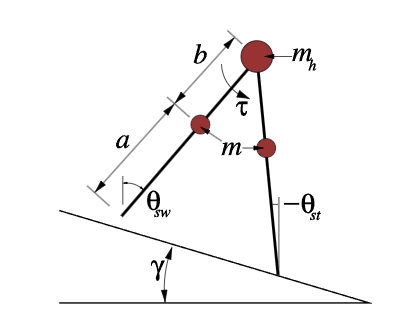
\includegraphics[width=8cm]{./figures/compassgaitmodel.png}
\caption{Schematic of the compass gait model. Angles $\theta_{sw}$ and $\theta_{st}$ are shown as the swing leg angle and stance leg angle, respectively.}
\label{fig:compassgaitmodel}
\end{figure}

% assumptions for model
In order to use the compass gait model a few assumptions must be made about the system. First, since the compass gait does not have the ability to bend at the hip, it must 
be assumed that during the swing, the swing leg retracts so that it does not collide with the ground during the swing phase. 
It is also assumed that a perfectly inelastic collision without sliding
occurs the instant the swing leg hits the ground. The compass gait is an extremely simple model, however it should be noted that physical models of the compass gait
have been built in \cite{article}.

% intro of eqs
In order to create a state space realization of the compass gait model a state matrix must be defined. For simplicity the swing and stance angles are renamed to
$x_1$ and $x_2$, respectively, with $x_3$ and $x_4$ being the anguar velocities of the swing and stance legs. The state matrix $\mb{X}$ is shown in equation
\ref{eq:statematrix}.

\begin{equation}
\label{eq:statematrix}
\mb{X} = 
\begin{bmatrix}
\\x_1\\
\\x_2\\
\\x_3\\
\\x_4\\
\end{bmatrix}, \quad
\begin{bmatrix}
\\x_3\\
\\x_4\\
\end{bmatrix}
 = 
\begin{bmatrix}
\\\dot{x_1}\\
\\\dot{x_2}\\
\end{bmatrix}
\end{equation}

The dynamic equations of the swing stage of the compass gait, from \cite{goswami:inria-00073701}, can be written in standard planar manupular dynamics form. 
This is shown in \ref{eq:swingeqn}, where $\mb{M}$, $\mb{N}$, and $\mb{G}$ are matrices shown in the appendix, and $\mb{U}$
 is the vector used to apply the torque to each leg, shown in
\ref{eq:U}.

\begin{equation}
\label{eq:swingeqn}
\mb{M(X)}\mb{\ddot{X}} + \mb{N(X, \dot{X})}\mb{\dot{X}} + \mb{G(X)} = \tau\mb{U}
\end{equation}

\begin{equation}
\label{eq:U}
\mb{U} = 
\begin{bmatrix}
\\1\\
\\-1\\
\\0\\
\\0\\
\end{bmatrix}
\end{equation}

Since heel strike (when the swing leg collides with the ground) is modeled as a perfectly inelastic 
collision, there is an instantaneous angular velocity change when heel stike occurs. Also, since the swing leg becomes the stance leg
after heel strike, the angles $x_1$ and $x_2$ must be switched in the mathematical model after each walking cycle. The transition matrices used to switch $x_1$ and $x_2$ as well 
as calculate the updated angular velocities after heel strike are shown in \ref{eq:trans1} and \ref{eq:trans2}, where $x^+$ represents the state
variable after heel strike and $x^-$ represents the state variable before impact, $\mb{Q^-}$ and $\mb{Q^+}$ are the angular velocity transition matrices shown in the appendix.

\begin{equation}
\label{eq:trans1}
\begin{bmatrix}
\\x_1^+\\
\\x_2^+\\
\end{bmatrix}
 = 
\begin{bmatrix}
0 & 1\\
1 & 0\\
\end{bmatrix}
\begin{bmatrix}
\\x_1^-\\
\\x_2^-\\
\end{bmatrix}
\end{equation}

\begin{equation}
\label{eq:trans2}
\mb{Q^+}
\begin{bmatrix}
\\x_3^+\\
\\x_4^+\\
\end{bmatrix}
 = 
\mb{Q^-}
\begin{bmatrix}
\\x_3^-\\
\\x_4^-\\
\end{bmatrix}
\end{equation}




\section{Natural Limit Cycles of the Passive Compass Gait}

It is important to define stability in the context of the compass gait for this paper. One possible meaning of stability in this context is that, while walking, 
the compass gait procedes forwards in a controlled manner and takes the same "path" for each walking cycle. Or perhaps stability could be mathematically defined
using Poincaré maps. While both of these definitions of stability are valid, stability in this paper simply refers to the ability of the compass gait system to 
continue walking forwards for the defined number of cycles.

When simulating the passive compass gait system, it can be observed that the stability of the compass gait is heavily dependent on the
given initial conditions and system parameters. It can also be observed that the basin of stability is extremely small and it is almost impossible
to "guess" the correct IC's and system parameters to create a stable walking system. This is one of the main issues of the compass gait.

When using stable initial conditions, the compass gait can be simulated over one or multiple walking cycles. Shown in Figure \ref{fig:onecycle}
is an example of a stable limit cycle for the compass gait over one walking cycle. As can be seen, the swing leg makes a large arc during the swing phase of the 
compass gait, while the stance leg pivots in place. The state variables during this walking cycle are also shown over time in Figure \ref{fig:states_onecycle}.

\begin{figure}[!h]
\centering
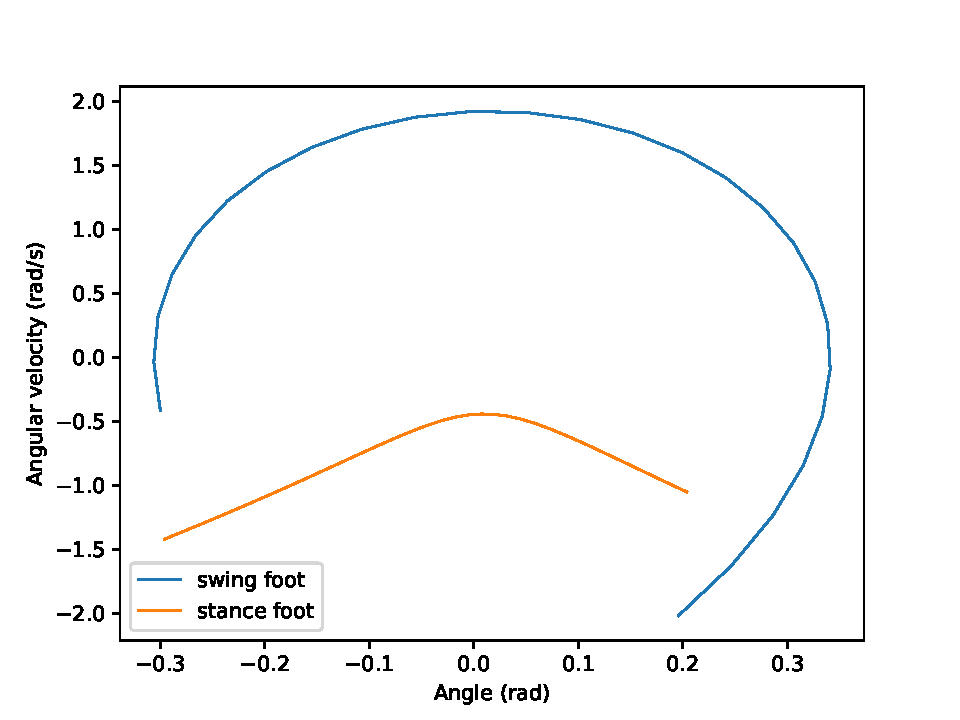
\includegraphics[width=10cm]{./figures/onecycle.pdf}
\caption{One walking limit cycle of the compass gait. The swing leg makes a large swing (shown in blue, a large cicle) around while the stance leg only pivots (shown in orange.)}
\label{fig:onecycle}
\end{figure}

\begin{figure}[h]
\centering
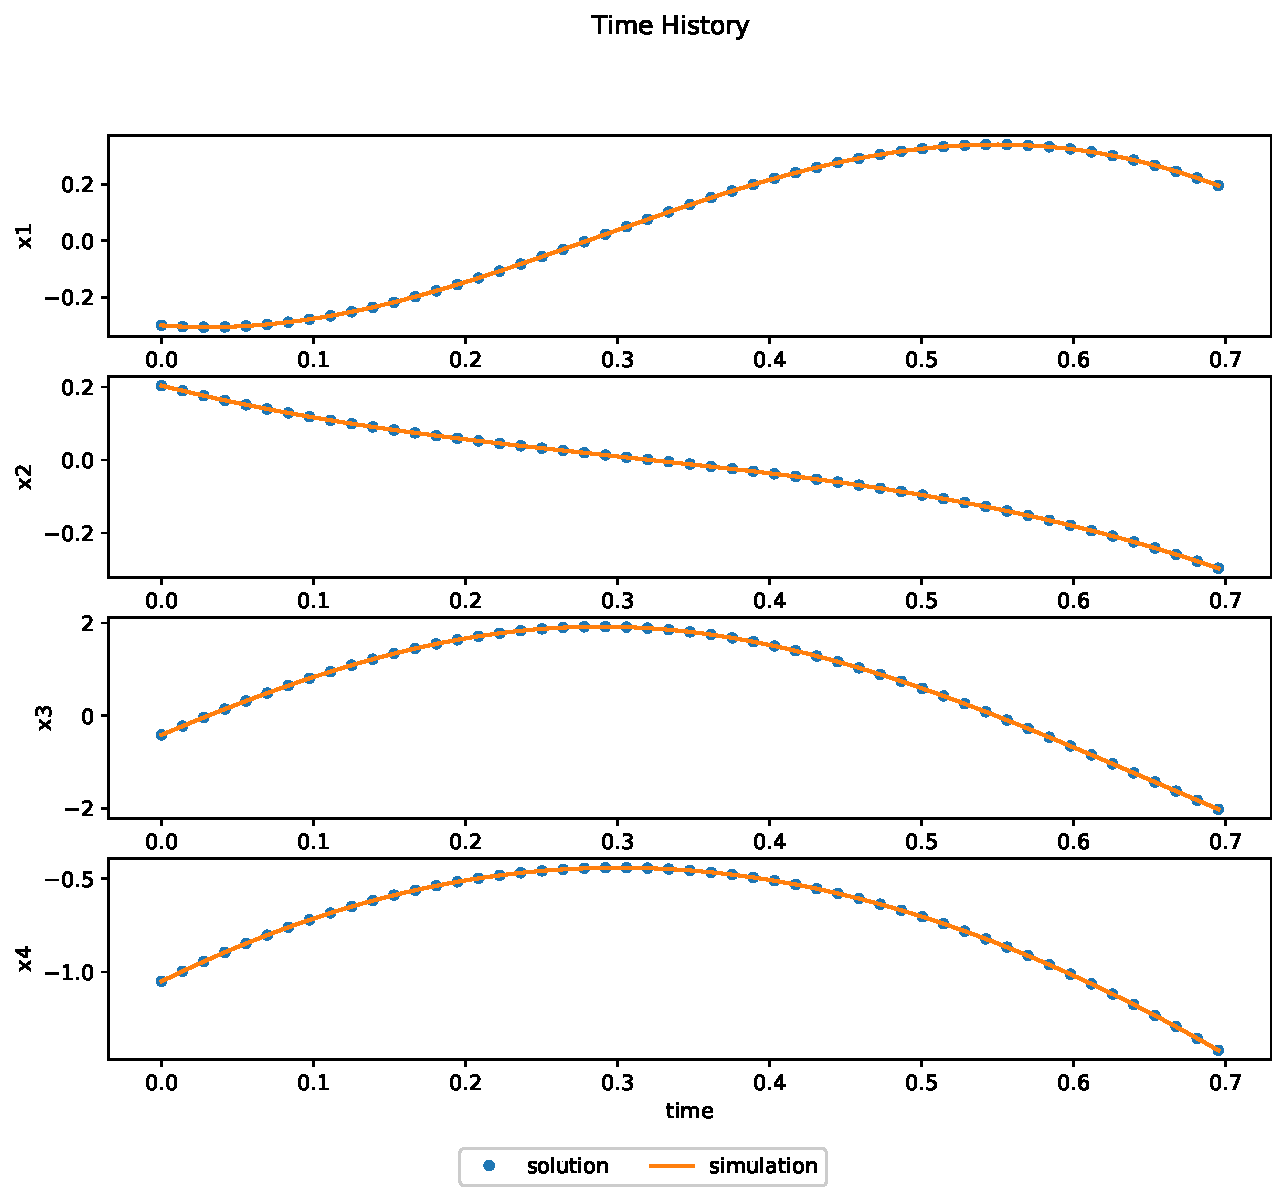
\includegraphics[width=9cm]{./figures/states_onecycle.pdf}
\caption{States of the compas gait over time for one walking cycle.}
\label{fig:states_onecycle}
\end{figure}

Figures \ref{fig:onecycle} and \ref{fig:states_onecycle} show the compass gait when stable initial conditions are used; however, most initial conditions
given to the compass gait system result in an unstable system. An example of a unstable gait is shown in Figure \ref{fig:unstable_onecycle}, where the initial angular velocities are 
not sufficent to overcome gravity, and the compass gait cannot start a cycle and will eventually fall down. It can be seen in this figure, that the swing leg initial angle 
is approximataly equal to the final angle of the swing leg, and the stance leg starts going forward, but runs out of momentum before falling backwards.

\begin{figure}[!h]
\centering
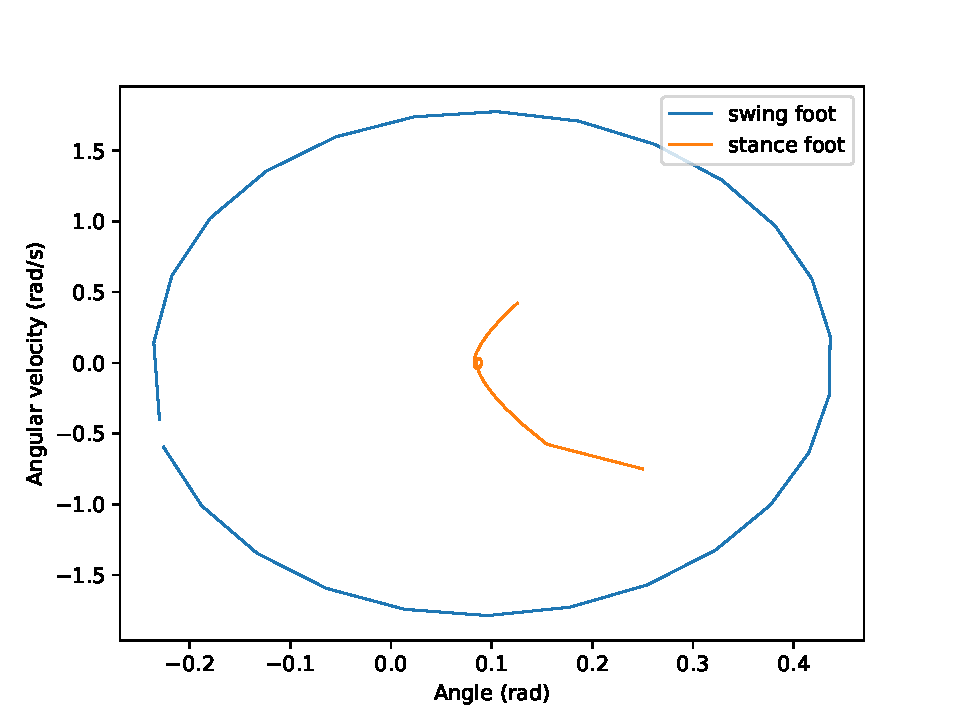
\includegraphics[width=10cm]{./figures/unstable_onecycle.pdf}
\caption{An example of an unstable limit cycle. In this case, the initial angular velocities make it impossible for the compass gait to start a walking cycle.}
\label{fig:unstable_onecycle}
\end{figure}

\clearpage

\section{Passive Optimization with Co-Design}

In order to acheive co-design with a simple passive compass gait system, an optimization problem was proposed.
This optimization problem, outlined in  \ref{eq:optprobsetup}, involved maximizing the point mass at the hip ($m_H$) in order to simulate the
compass gait robot "carrying" a heavy object. In order to acheive this goal, the lengths below and above the leg point mass, a and b, were optimized.
The leg point mass ($m$) also changed based on the total length of the legs based on the given density of the legs.

\begin{equation}
\begin{aligned}
\text{Objective: Maximize $m_H$}\\
\text{Subject to:}\\
\text{Dynamic Constraints of System}\\
\text{Design Variables: 0.1$<$a$<$1, 0.1$<$b$<$1, (m)}\\
\text{Hip Mass: 5$<$$m_H$$<$80, (kg)}\\
\text{Leg Mass: } m = 5(a+b), \text{(kg)}\\
\text{End States $x_1$ and $x_2$ are Constrained Based on Trajectory Generation}
\end{aligned}
\label{eq:optprobsetup}
\end{equation}


The goal of this optimization problem was to increase the range of initial conditions that caused the compass gait to complete one stable cycle
while maximizing the mass at the hip. In order to acheive this goal a trajectory generation method was used, where the compass gait model was
first simulated using known stable initial conditions and system parameters and the final position states ($x_1$ and $x_2$) were recorded and passed to the optimization
model. The final position states of the optimization model were constrained to be equal to the recorded final position states found in the trajectory generation
simulation. This gave the the compass gait optimization problem a goal to acheive in order to keep the system stable. Figure \ref{fig:optlogicdiagram} shows a diagram
outlining this process.

\begin{figure}[h]
\setlength{\unitlength}{0.14in} % selecting unit length
\centering % used for centering Figure
\begin{picture}(32,15) % picture environment with the size (dimensions)
% 32 length units wide, and 15 units high.
\put(0,5.5){\vector(1,0){5}}
\put(5,3.25){\framebox(10,5){Trajectory Generation}}
\put(20.2,3.25){\framebox(10,5){Optimization Problem}}
\put(15,5.5){\vector(1,0){5.2}}
\put(30.2,5.5){\vector(1,0){12}}
\put(25.2, 12){\vector(0,-1){3.7}}
\put(0,6){Stable IC's}
\put(15.2, 6){End States}
\put(15.3, 4.5){$x_1$ and $x_2$}
\put(30.4, 6){Stable, optimized system}
\put(23.3, 12.2){New IC's}
\end{picture}
\caption{A trajectory generation method was used where a system with stable initial conditions found end states ($x_1$ and $x_2$) to be used for the optimization problem.} % title of the Figure
\label{fig:optlogicdiagram} % label to refer figure in text
\end{figure}
  

While it was not possible to make all initial conditions stable without a controller, the range of initial conditions was
increased. Shown in Figure \ref{fig:nonoptlimcycle} is the limit cycle of the compass gait without optimization with the initial conditions and system parameters 
shown in Table \ref{tab:nonoptparam}. As can be seen, the compass gait system is not able to complete a full cycle and can be said to be unstable.

\begin{figure}[h]
\centering
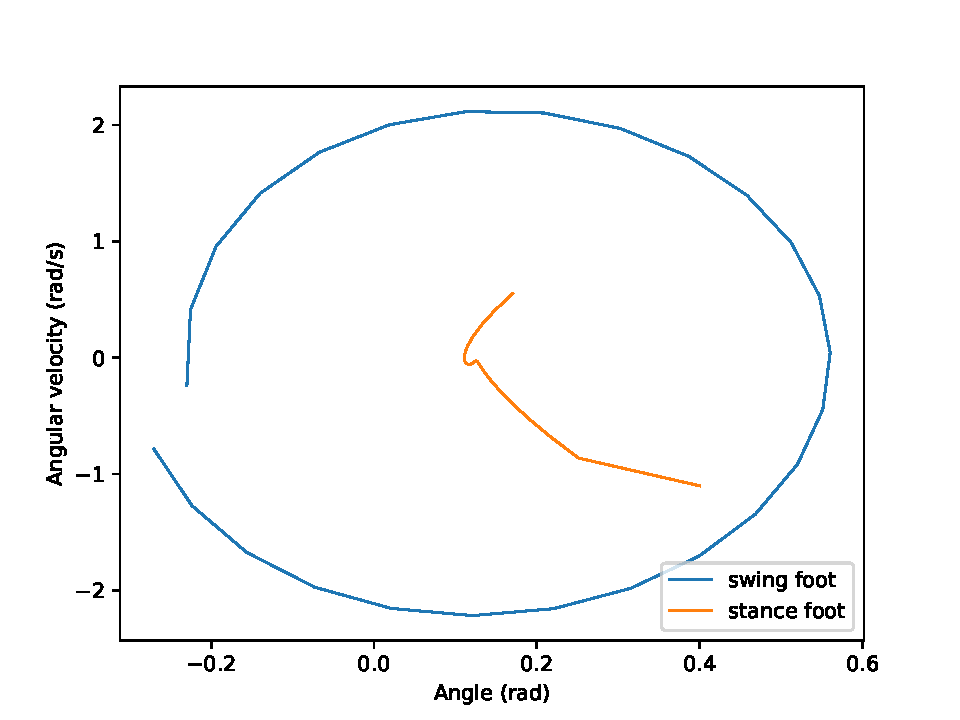
\includegraphics[width=10cm]{./figures/nonopt_limitcycle.pdf}
\caption{Limit cycle of the non optimized compass gait over one cycle with the same initial conditions as the optimized system. It can be seen that the system does not 
complete a full cycle.}
\label{fig:nonoptlimcycle}
\end{figure}

\begin{table}[h]
\centering
\caption{Initial Conditions and System Parameters of the Non-Optimized Compass Gait Shown in \ref{fig:nonoptlimcycle}}
\begin{tabular}{lr}
\toprule
Parameter & Value \\
\midrule
$m (kg)$ & 5 \\
$m_H (kg)$ & 10 \\
$a (m)$ & 0.5 \\
$b (m)$ & 0.5 \\
$\gamma (slope, rad)$ & 0.05 \\
$x_1 (rad)$ & -0.23 \\
$x_2 (rad)$ & 0.4 \\
$x_3 (rad/s)$ & -0.24 \\
$x_4 (rad/s)$ & -1.1 \\
\bottomrule
\end{tabular}
\label{tab:nonoptparam}
\end{table}

The limit cycle of the non-optimized system can be compared to that of the optimized system in order to see the benefits of the optimization.
Shown in Figure \ref{fig:passiveopt} is the limit cycle of the optimized compass gait system with the same initial conditions as the non-optimized compass gait.
It can be seen that after optimization, the system completes a full stable walking cycle.
The optimized system parameters of the new system are shown in Table \ref{tab:optparam}. Not only can it be seen that the compass gait system gained stability from the 
optimization, but it also succesfully maximized the mass at the hip.

\begin{figure}[h]
\centering
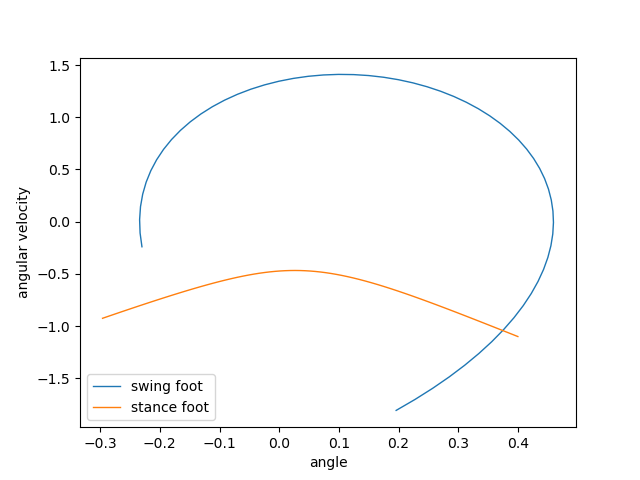
\includegraphics[width=10cm]{./figures/passiveopt_limitcycle.png}
\caption{The limit cycle of the optimized compass gait. It can be seen that the system is stable for the first walking cycle.}
\label{fig:passiveopt}
\end{figure}

\begin{table}[h]
\centering
\caption{Optimized System Parameters of the compass gait.}
\begin{tabular}{lr}
\toprule
Parameter & Value \\
\midrule
$m (kg)$ & 8.96 \\
$m_H (kg)$ & 80 \\
$a (m)$ & 0.83 \\
$b (m)$ & 0.957 \\
\bottomrule
\end{tabular}
\label{tab:optparam}
\end{table}

While this optimization problem was succesful, it has its limitations. First, as previously mentioned, without a using an active controller
it is impossible to guarentee that all initial conditions for the compass gait will result in a stable walking limit cycle. Also, it is desired that the optimized
compass gait system complete multiple walking cycles instead of just one. In order to fix these two limitation, active CCD can be used to optimize the problem 
and simulate the compass gait over any given number of walking cycles.

\clearpage

\section{Active Control Co-Design of the Compass Gait}

In order to perform Active CCD on the compass gait a torque controller was activated at the hip. The addition of this torque controller allowed
for the problem to be optimized to a more meaningful cost function. Instead of simply optimizing the hip mass of the compass gait, the time per cycle 
and the total torque used was minimized. The cost function used is shown in \ref{eq:costfunc}, where $\tau_r$ and $t_r$ are reference scalers used 
to normalize $\tau$ and $t$. The values of $\tau_r$ and $t_r$ which were used are shown in \ref{eq:refvars}

\begin{equation}
\label{eq:costfunc}
J = 
\int_{0}^{t} (\tau / \tau_r)^2 + (t/t_r) \,dt 
\end{equation}

\begin{equation}
\label{eq:refvars}
\tau_r = 6.32 (N*m), 
t_r = 0.5 (s)
\end{equation}

Since the hip mass was no longer part of the cost function, it was chosen to also 
be a design variable of the system. The constraints of the system remained the same, outlined in \ref{eq:OLprob}.

\begin{equation}
\begin{aligned}
\text{Minimize: } J = \int_{0}^{t} (\tau / \tau_r)^2 + (t/t_r) \,dt \\
\text{Subject to:}\\
\text{Dynamic Constraints of System}\\
\text{Design Variables: } 0.1<a<1 (m), 0.1<b<1 (m), 0<m_H<100 \text{kg}\\
\text{Leg Mass: } m = 5(a+b)\\
\text{End States of $x_1$ and $x_2$ Constrained by Trajectory Generation}
\end{aligned}
\label{eq:OLprob}
\end{equation}

In order to optimize the compass gait through multiple walking cycles and ensure stability, the trajectory generation method used
in the previous section was used with continued simulation of the system after the first cycle.
After the trajectory generation was performed and the final states of the system were determined, CCD was performed on the system in order to
optimize the design variables and the torque over one walking cycle. After the optimal values for the design variables were determined, the system was 
simulated for a fixed number of cycles with trajectory optimization (torque optimization) according to the set cost function. Figure \ref{fig:OLblock}
shows a diagram outlining the new trajectory optimization process.

\begin{figure}[h]
\setlength{\unitlength}{0.14in} % selecting unit length
\centering % used for centering Figure
\begin{picture}(32,15) % picture environment with the size (dimensions)
% 32 length units wide, and 15 units high.
\put(0,5.5){\vector(1,0){5}}
\put(5,3.25){\framebox(10,5){Trajectory Generation}}
\put(20.2,3.25){\framebox(8,5){CCD For 1 Cycle}}
\put(30.2,3.25){\framebox(12,5){Simulation with Torue Opt.}}
\put(15,5.5){\vector(1,0){5.2}}
\put(28.2,5.5){\vector(1,0){2}}
\put(25.2, 12){\vector(0,-1){3.7}}
\put(10, 3.25){\vector(0,-1){2}}
\put(10, 1.25){\vector(1, 0){26.2}}
\put(36.2, 1.25){\vector(0, 1){2}}
\put(0,6){Stable IC's}
\put(15.2, 6){End States}
\put(15.3, 4.5){$x_1$ and $x_2$}
\put(23.3, 12.2){New IC's}
\put(18, 1.5){End States $x_1$ and $x_2$}
\end{picture}
\caption{The trajectory generation method used in the previous example was used with continued trajectory optimization after one cycle.} % title of the Figure
\label{fig:OLblock} % label to refer figure in text
\end{figure}

In order to compare the compass gaits performance when CCD is used to other compass gait scenarios, three simulations were ran and compared:
The comass gait with active CCD (Figure \ref{fig:OLblock}), the compass gait with active open loop control without co-design, and the non-optimized passive compass gait system.
Each of these systems were simulated over 10 cycles and the stability, total torque used, time per cycle, and optimized design variables were compared. Each system used the initial conditions and 
system parameters shown in Table \ref{tab:params}.

\begin{table}[h]
\centering
\caption{Initial Conditions and System Parameters Used to Simulate the Compass Gait.}
\begin{tabular}{lr}
\toprule
Parameter & Value \\
\midrule
$m (kg)$ & 5 \\
$m_H (kg)$ & 10 \\
$a (m)$ & 0.5 \\
$b (m)$ & 0.5 \\
$\gamma (slope, rad)$ & 0.05 \\
$x_1 (rad)$ & -0.3 \\
$x_2 (rad)$ & 0.2038 \\
$x_3 (rad/s)$ & -0.41215 \\
$x_4 (rad/s)$ & -1.0501 \\
\end{tabular}
\label{tab:params}
\end{table}

Shown in Figures \ref{fig:limcyc_passive} and \ref{fig:timehis_passive} are the limit cycle and total time history of the state variables for the passive compass gait system when simulated using the 
given initial conditions and system parameters. As can be seen the chosen initial conditions resulted in a stable, well behaved system for the passive compass gait. It can be 
seen that it takes about three cycles for the system to converge to a single limit cycle; however, there still exists some oscilitations in the limit cycle.

\begin{figure}[h]
\centering
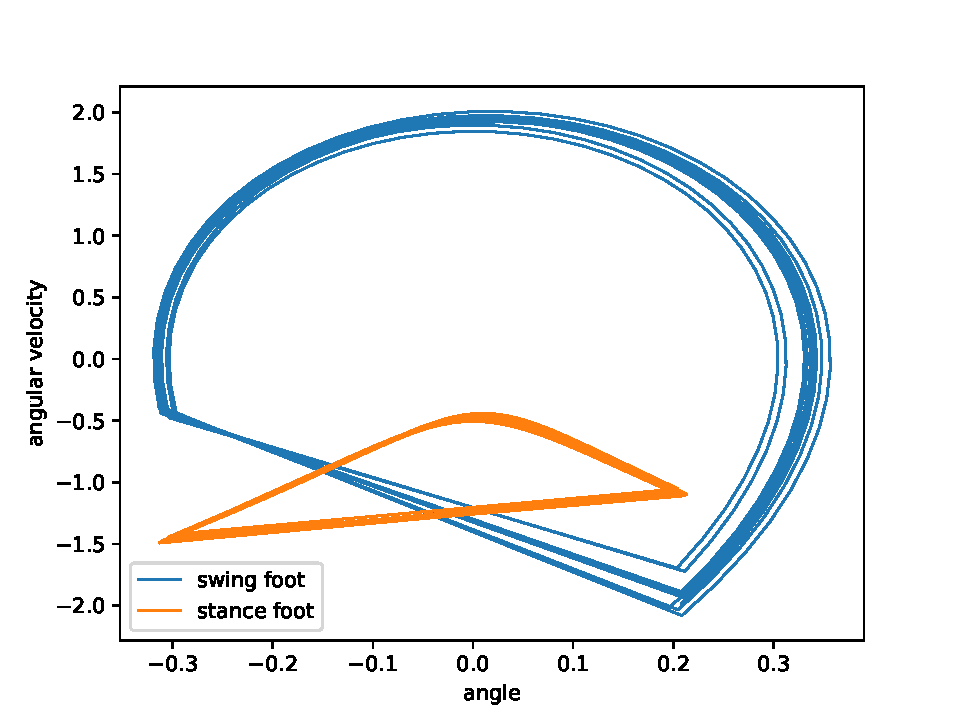
\includegraphics[width=8cm]{./figures/limitcycle_passivesim.pdf}
\caption{The limit cycle of the passive compass gait over 10 cycles.}
\label{fig:limcyc_passive}
\end{figure}

\begin{figure}[h]
\centering
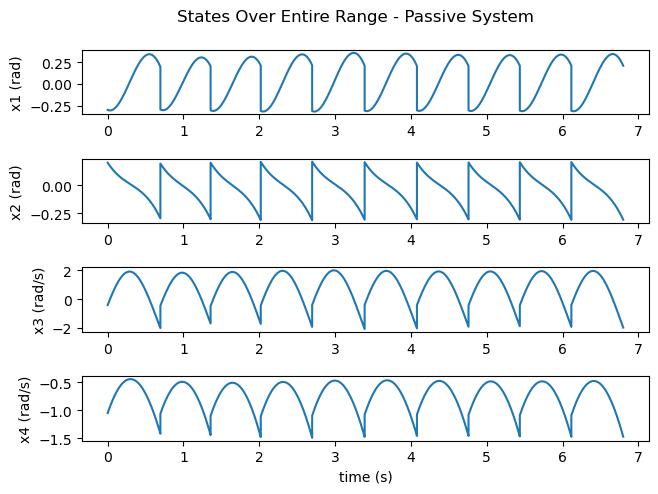
\includegraphics[width=8cm]{./figures/timehis_passivesim.png}
\caption{The total time history of the state variables of the passive compass gait over 10 cycles.}
\label{fig:timehis_passive}
\end{figure}

Similarly, shown in Figures \ref{fig:lim_noco} and \ref{fig:timehis_noco} are the limit cycle and total time history of the state variables and controls for the compass gait 
using active open loop control without co-design. The same trajectory generation method was used during this simulation, except without co-design (only torque optimization).
It can be seen that it takes approximataly 6 cycles to converge to a single limit cycle; also, the indivual walking cycles are much more spaced out when compared to the passive system.
However, the final limit cycle is much smaller than that of the passive limit cycle, resulting in less time per cycle. This can be seen when comparing the total time history of the 
active system without co-design to the passive system; the average time per cycle and total time of the active system is smaller than that of the passive system.

\begin{figure}[h]
\centering
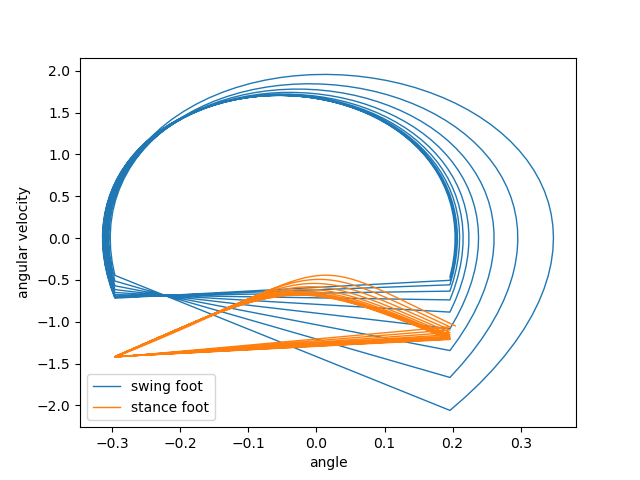
\includegraphics[width=8cm]{./figures/limcycle_nocodesign.png}
\caption{The limit cycle of the active compass gait using open loop control without co-design.}
\label{fig:lim_noco}
\end{figure}

\begin{figure}[h]
\centering
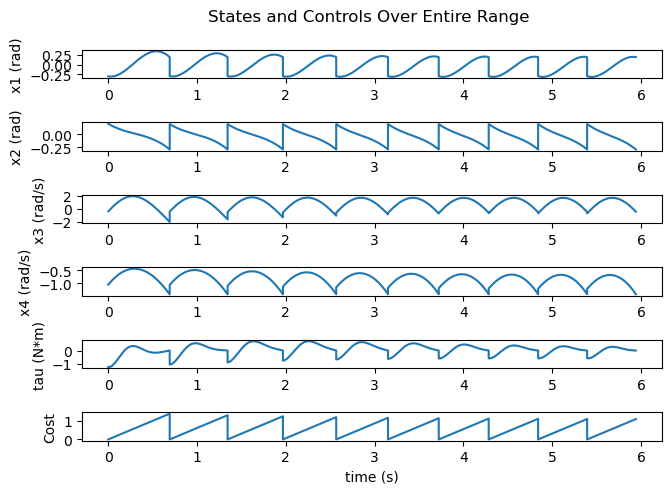
\includegraphics[width=8cm]{./figures/timehis_nocodesign.png}
\caption{The total time history of the state variables, control, and cost of the active compass gait without co-design.}
\label{fig:timehis_noco}
\end{figure}

Finally, the limit cycle and total time history of the compass gait when CCD is used is shown in Figures \ref{fig:limcyc_CCD} and \ref{fig:timehis_CCD}. When comparing the limit 
cycle of the CCD compass gait to the other two systems, it can be seen that one small waliking cycle is performed before converging into the final limit cycle in approximataly 4 
iterations. It can also be seen from the time history that the CCD compass gait has a smaller time per cycle than both the passive system and the open loop system without co-design. 
It can also be seen that much less torque is used to control the system than the compass gait without co-design.

Shown in Table \ref{tab:opt_vars} are the optimized design variables found using CCD with the compass gait system. As can be seen, in order to reduce torque and time per cycle, 
the system prefers to have a higher mass at the hip and a longer leg segment below the point mass on the leg. In order to determine the best design variables for a system, 
the bounds of the design variables should be adjusted as desired.

\begin{table}[h]
\centering
\caption{Optimized Design Variables Found Using CCD}
\begin{tabular}{lr}
\toprule
Parameter & Value \\
\midrule
$m (kg)$ & 6.45 \\
$m_H (kg)$ & 100 \\
$a (m)$ & 1 \\
$b (m)$ & 0.29 \\
\end{tabular}
\label{tab:opt_vars}
\end{table}
  


\begin{figure}[h]
\centering
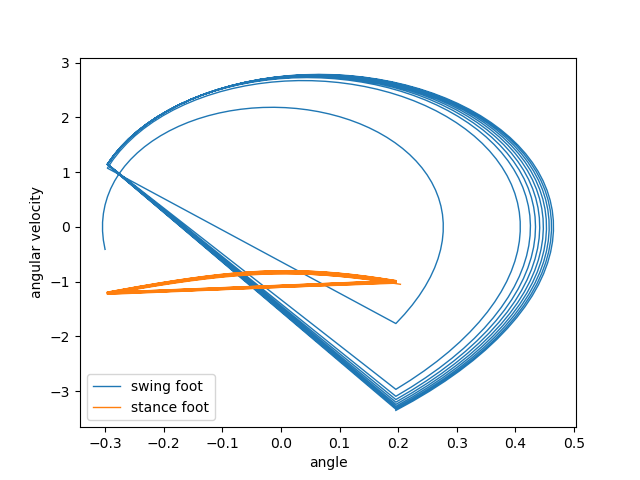
\includegraphics[width=8cm]{./figures/limcyc_CCD.png}
\caption{The limit cycle of the compass gait when CCD is used.}
\label{fig:limcyc_CCD}
\end{figure}

\begin{figure}[h]
\centering
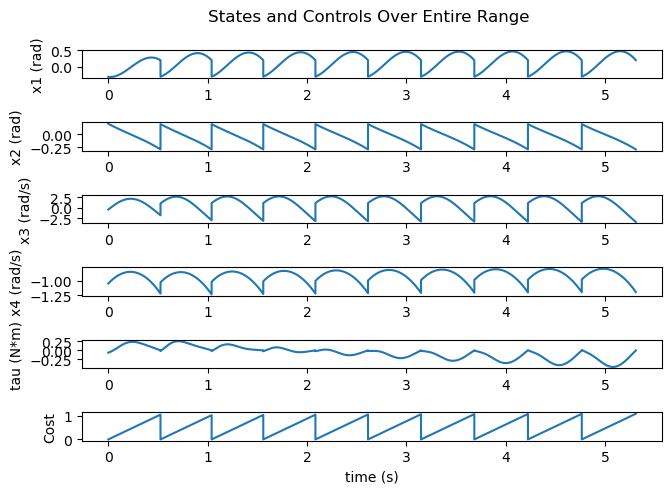
\includegraphics[width=8cm]{./figures/timehis_CCD.png}
\caption{The total time history of the state variables, control, and cost when CCD is used.}
\label{fig:timehis_CCD}
\end{figure}  


Shown in Table \ref{tab:time} is the average time per cycle and the total time to complete 10 cycles for each compass gait system which was simulated. As can be seen, the CCD system 
has the shortest average time per cycle and total time, followed by the open loop system without control, then the passive system. From these results it can be said that 
CCD is more effective in reducing the time per cycle of the compass gait than control without co-design, and any control at all is much better than a passive system.

\begin{table}[h]
\centering
\caption{Average Time per Cycle and Total Time for 10 Cycles of Each Simulation (seconds)}
\begin{tabular}{cccc}
\toprule
Simulation & Average Time/Cycle & Total Time & Percent Improvement\\
\midrule
Passive System & 0.680 & 6.8 & N/A\\
Active System Without Co-Design & 0.594 & 5.94 & 12.66$\%$ \\
System with CCD & 0.531 & 5.31 & 21.91$\%$\\
\end{tabular}
\label{tab:time}
\end{table}

The total torque used during the simulations of the compass gait with CCD and the open loop system without co-design can also be compared. Shown in Table \ref{tab:tautot} is 
the summation of the square of $\tau$ over all 10 cycles, this is shown in equation \ref{eq:summation}. From the table, It can be seen that much more torque is needed to control 
the non-optimized 
compass gait when compared to the compass gait with CCD. From the results found in these simulations, it can be concluded that using CCD with the compass gait 
system can greatly decrease the cost of control when compared to compass gait systems without co-design or optimization.

\begin{equation}
\label{eq:summation}
\tau_{sum} = 
\sum_{t = 0}^{t = t_f}
\tau^2
\end{equation}

\begin{table}[h]
\centering
\caption{Summation of $\tau^2$ for the CCD and Open Loop Control System}
\begin{tabular}{ccc}
\toprule
System & $\sum \tau^2$ & Percent Improvement \\
\midrule
Active System Without Co-Design & 133.46 & N/A\\
System with CCD & 29.17 & 78.1$\%$\\
\end{tabular}
\label{tab:tautot}
\end{table}


\section{Conclusions and Future Works}

During this study, CCD was applied to the compass gait bipedal robot and the system was optimized first to maximize the mass at the hip with a passive system, 
then to minimize the torque used and time per cycle with a torque controller at the hip. A trajectory generation method was also used in this paper, 
where a passive system is first simulated with stable initial conditions and the end states ($x_1$ and $x_2$) are used during the optimization process in order to 
ensure a stable system.

From the passive optimization, it was shown that not only can optimization 
of the design variables in the compass gait allow for the hip mass to be maximized, but the optimization can also allow for a greater range of initial conditions 
which result in a stable first walking cycle. It was shown that when the optimized compass gait was given the same initial conditions which would typically 
result in an unstable walking cycle with a non-optimized passive system, the system parameters were optimized so that the compass gait had a stable first walking cycle 
while still maximizing the hip mass.

When CCD was used on the active compass gait, it was shown that the cost of control was reduced by 10.83$\%$ when compared to a system 
with open loop control without co-design using the same intial conditions and system parameters. Shown in Table \ref{tab:costofcon} is the total cost of control over 10 
walking cycles when CCD is used compared to active control without co-design. The cost shown is the same cost function shown above in equation \ref{eq:costfunc}. CCD reduced the 
cost by reducing the torque used and time per cycle in accordance with the cost function. The compass gait with CCD used only 21.8$\%$ as much torque as the system without co-design 
and the time per cycle was reduced by 0.063 seconds, or 10.6$\%$.

\begin{table}[h]
\centering
\caption{Cost of Control for the CCD Compass Gait vs Only Open Loop Control}
\begin{tabular}{lr}
\toprule
System & Cost of Control \\
\midrule
Active System Without Co-Design & 11.91\\
System with CCD & 10.62\\
Percent Improvement & 10.83$\%$ \\
\end{tabular}
\label{tab:costofcon}
\end{table}

One of the main limitations of this study is that CCD was applied to the compass gait over only one walking cycle using the trajectory generation method,
then the compass gait was simulated with open-loop 
control for the given number of cycles.
Ideally, when using CCD for a system with cyclic behavior it would be desired that the system parameters be optimized based on the entire trajectory of the system 
(over all cycles); however, due to the structure of the Dymos code, it was only possible to optimize the first walking cycle of the compass gait during this study. 
In future studies, the compass gait should be optimized over the entire trajectory in order to obtain the best possible system parameters for the system.

Another future study which should be conducted is the use of a closed loop control algorithm in order used to perform CCD. One example of this is using 
MPC or LQR control in order to optimize and control the compass gait. The use of closed loop CCD with the compass would result in more optimal system parameters 
and better trajectory optimization. 

\clearpage
\appendix

\section{Compass Gait Equations}

Shown in this appendix is a more complete version of the dynamics equations of the compass gait. The swing stage dynamics can be written in standard planar manipulator 
dynamics form, shown in \ref{eq:swingeq}. The $\mb{M}$, $\mb{N}$, $\mb{G}$, and $\mb{U2}$ matrices are also shown in \ref{eq:M}, \ref{eq:N}, \ref{eq:G}, and \ref{eq:U} respectively.

\begin{equation}
\label{eq:swingeq}
\mb{M(X)}\mb{\ddot{X}} + \mb{N(X, \dot{X})}\mb{\dot{X}} + \mb{G(X)} = \tau\mb{U}
\end{equation}

\begin{equation}
\mb{M} = 
\label{eq:M}
\begin{bmatrix}
\\mb^2 &  -mlbcos(x_2 - x_1)\\
\\-mlbcos(x_2 - x_1) &  m_{H}l^2 + m(l^2 + a^2)\\
\end{bmatrix}
\end{equation}

\begin{equation}
\mb{N} = 
\label{eq:N}
\begin{bmatrix}
\\0 &  mlb\dot{x_2}sin(x_2 - x_1)\\
\\-mlb\dot{x_1}sin(x_2 - x_1) &  0\\
\end{bmatrix}
\end{equation}

\begin{equation}
\mb{G} = 
\label{eq:G}
\begin{bmatrix}
\\mgbsin(x_1)\\
\\-(m_{H}l + m(a+l))gsin(x_2)\\
\end{bmatrix}
\end{equation}

\begin{equation}
\mb{U} = 
\label{eq:U2}
\begin{bmatrix}
\\1\\
\\-1\\
\\0\\
\\0\\
\end{bmatrix}
\end{equation}



The transition equations when heel strike occurs are shown in \ref{eq:transeqn} and \ref{eq:transeqn2}, where $x^+$ signifies a state variables after heel strike and $x^-$ 
signals a state variable before
heel strike. The transition matrices $\mb{Q^+}$ and $\mb{Q^-}$ are shown in \ref{eq:Q-} and \ref{}. Note that $\alpha$ represents half the angle between the swing and stance 
legs.

\begin{equation}
\label{eq:transeqn}
\begin{bmatrix}
\\x_1^+\\
\\x_2^+\\
\end{bmatrix}
 = 
\begin{bmatrix}
0 & 1\\
1 & 0\\
\end{bmatrix}
\begin{bmatrix}
\\x_1^-\\
\\x_2^-\\
\end{bmatrix}
\end{equation}

\begin{equation}
\label{eq:transeqn2}
\mb{Q^+}
\begin{bmatrix}
\\x_3^+\\
\\x_4^+\\
\end{bmatrix}
= 
\mb{Q^-}
\begin{bmatrix}
\\x_3^-\\
\\x_4^-\\
\end{bmatrix}
\end{equation}

\begin{equation}
\mb{Q^-} = 
\label{eq:Q-}
\begin{bmatrix}
\\-mab & -mab + (m_Hl^2+2mal)cos(2\alpha)\\
\\0 & -mab\\
\end{bmatrix}
\end{equation}

\begin{equation}
\mb{Q^+} = 
\label{eq:Q+}
\begin{bmatrix}
\\mb(b-lcos(2\alpha)) & ml(l-bcos(2\alpha)) + ma^2 + m_Hl^2\\
\\mb^2 & -mblcos(2\alpha)\\
\end{bmatrix}
\end{equation}

\bibliography{bib/references}
\bibliographystyle{plain}

\end{document}
